% ***********************************************
%***********COSAS A MEJORAR O CORREGIR***********
%-A�adir gr�fica en la soluci�n del ej 7
%-Cambiar para que todas las gr�ficas se use X para polos y O para ceros
%
%
%
% ***********************************************
% Preamble
% ---
\documentclass[10pt,a4paper]{article}

% Packages
% ---
\usepackage[latin1]{inputenc}
\usepackage{amsmath}
\usepackage{mathtools}
\usepackage{amsfonts}
\usepackage{amssymb}
\usepackage{layout}
\usepackage{graphics}
\usepackage{graphicx}
\usepackage[spanish]{babel}
\usepackage{lastpage}
\usepackage{tabto}
\usepackage{xcolor}
\usepackage[a4paper, top=1 in,bottom=1in, left=1 in, right=0.7 in]{geometry}
\usepackage{fancyhdr}
\pagestyle{fancy}
\usepackage{mdwlist}
\usepackage{comment}

%ELEGIR VERSION 
%Comentar para eliminar la solucion de todos los ejercicios y dejar la version para los 
% alumnos, a saber con un solo punto resuelto por ejercicio.

%\includecomment{profesor}    % version profesor
\excludecomment{profesor}	  % version alumnos

\lhead{\footnotesize An\'alisis de Se\~nales y Sistemas - A\~no \the\year{} Ver. 2021.11.19}
\chead{}
\rhead{\footnotesize Trabajo Pr\'actico N$^\text o$3: Integrales Complejas.}
\lfoot{}
\cfoot{}
\rfoot{\footnotesize P\'agina \thepage\ de \pageref{LastPage}}
\renewcommand{\headrulewidth}{0.4pt}
\renewcommand{\footrulewidth}{0.4pt}

\title{
	\textsc{
\includegraphics[width=0.55\textwidth]{logoUTN.jpg}} ~\\
	{\large Departamento de Electr\'onica}\\ 
	[0.1cm]
	{\Huge{An\'alisis de Se\~nales y Sistemas}} \\
	[0.25cm]
	{\Large{Trabajo Pr\'{a}ctico N$^{\text {o}}$3: Integrales Complejas}		\\
	}}
\author{}
\date{}

% Main document ********************************************
% ---
\begin{document}
\maketitle
\begin{profesor}
	\hspace{6cm}(Versi�n PROFESOR)
\end{profesor}
\thispagestyle{fancy}

\section*{Enunciados:}
\label{sec:enun}
% ***********************************************
% 					Ejercicio 1
% ***********************************************
\begin{enumerate}
\item {Hallar una representaci\'on de $z=z(t)$ para los segmentos rectil�neos cuyos extremos se dan a continuaci\'on:}
\begin{enumerate}
	\item $z=0$ y $z=-2+10i$ \tab Rta: $x=-t$, $y=5t$ ~ $\forall t:0\leq t\leq 2.$ % (a)
	\item $z=-3+2i$	y $z=-4+5i$	**\tab Rta: $x=-t$, $y=3t-7$ ~ $\forall t:3\leq t\leq 4.$	% (b)
	\item $z=2i$ y $z=5+17i$ \tab Rta: $x=t$, $y=3t+2$ ~ $\forall t:0\leq t \leq 5.$ % (c)
	\item $z=1$ y $z=i$ **\tab Rta: $x=1-t$, $y=t$ ~ $\forall t:0\leq t \leq 1.$ % (d)
\end{enumerate}


% ***********************************************
% 					Ejercicio 2
% ***********************************************
\item {Determinar las curvas representadas por las funciones dadas:}
\begin{enumerate}
	\item % (a)
	$5-i2t \quad \forall t:  -1 \leq t \leq 1$ ** \tab Rta: Segmento rectil\'ineo 
	entre $z=5+2i$ \\ \phantom{.} \tab y $z=5-2i$	
	\item % (b)
	$1-i+2e^{i\theta} \quad \forall t: 0 \leq \theta \leq \pi $ **		 \tab 
	Rta: Semic\'irculo superior de la circunferencia \\ 
	\phantom{.} \tab centrada en $z_0=1-i$ y radio $\rho =2$
\end{enumerate}

% ***********************************************
% 					Ejercicio 3
% ***********************************************
\item {Determinar el valor de las siguientes integrales:}	
		
\begin{enumerate}
	\item % (a)
	$ \int_{(0,0)}^{(1,1)} Re\{z\} dz $	siguiendo las trayectorias C\textsubscript{1}, 
	C\textsubscript{2} y C\textsubscript{3} mostradas en la figura, 
	desde el origen hasta el punto de coordenadas $(1+i)$.
	
	\begin{figure}[!htbp]
		\centering
		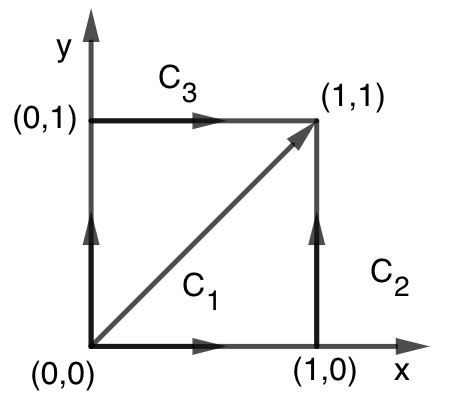
\includegraphics[width=4cm]{tp3_3a.png}
		\label{fig:ej3a}
	\end{figure}

	Rta:	C\textsubscript1: $I=\frac{1}{2}+\frac{1}{2}i$; C\textsubscript2: $I=\frac{1}{2}+i$; C\textsubscript3: $I=\frac{1}{2}$
	
	\item % (b)
	$ \int_{(0,0)}^{(1,1)} (y-x-i3x^2)dz $	siguiendo las trayectorias $C_1$ y $C_3$
	desde el origen hasta el punto de coordenadas $(1+i)$. ** 	\\
	Rta: $C_1$: $I=1-i$; $C_3$: $I=\frac{1}{2}(1-i)$.									

	\item % (c)
	$ \int_{(0,0)}^{(2,4)}(z^2)dz $ siguiendo las trayectorias $C_4$, $C_5$ o $C_6$ desde el origen al punto de coordenadas $(2+4i)$. \\
	Rta: $I=-\frac{88}{3}-i\frac{16}{3}=-29.33-i5.33$.									

	\begin{figure}[!htbp]
		\centering
		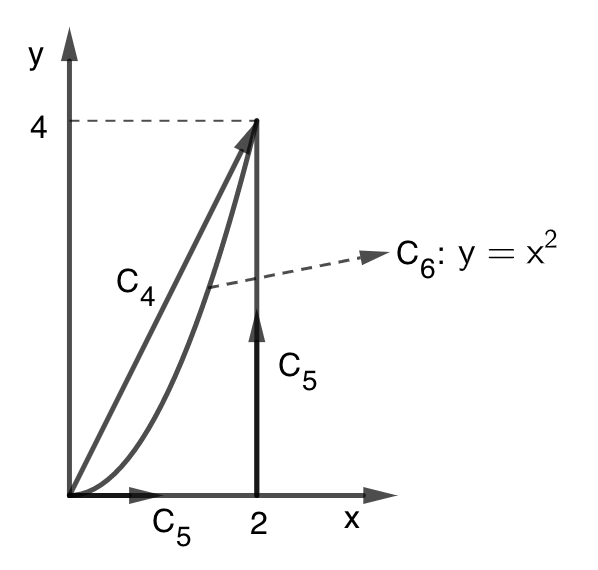
\includegraphics[width=5cm]{tp3_3c.png}
		\label{fig:ej3c}
	\end{figure}

\end{enumerate}

% ***********************************************
%					Ejercicio 4
% ***********************************************
\item {Si $C_7$ es la curva $y=4x-1$ que une los puntos $(0,-1)$ a $(1,3)$ del 
plano complejo, determinar el valor de $\int_{C_7}^{}(z^2-4zi) dz$. \tab Rta: 
$I=\frac{10}{3}+i\frac{23}{3}$}

% ***********************************************
% 					Ejercicio 5
% ***********************************************
\item {Integrar $\int_{C_6}(z+1)dz$ desde el origen hasta el punto $(1,1)$ 
siguiendo la trayectoria $C_6$: $y=x^2$. ** \tab Rta: $I=1+2i$.}	

% ***********************************************
% 					Ejercicio 6
% ***********************************************
\item {Integrar $\oint_{C}z^2dz$ a lo largo de los segmentos que unen $1+0i$ 
con 
$0+1i$, luego $0+1i$ con $0-1i$, y finalmente $0-1i$ con $1+0i$. \tab Rta: 
$I=0$.}	

	\begin{figure}[!htbp]
		\centering
		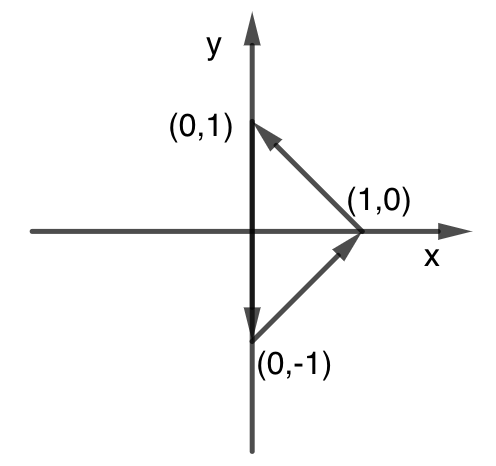
\includegraphics[width=4.5cm]{tp3_6.png}
		\label{fig:ej3a}
	\end{figure}

\suspend{enumerate}
Resolver las siguientes integrales aplicando la \textbf{F\'ormula de la Integral de Cauchy}
\resume{enumerate}
% ***********************************************
% 					Ejercicio 7
% ***********************************************
\item Integrar la funci\'on $f(z)=\frac{z^2-2z}{z^2+4}$ alrededor de la curva indicada:
\begin{enumerate}
	\item $|z-i|=2$ \tab Rta: $I=-2\pi (1+i)$
	\item $\left| z+\frac{1}{2}\right| =1$ ** \tab Rta: $I=0$
	\item $|z+1+i|=2$ \tab Rta: $I=2\pi (1-i)$
	\item $|z+2-i|=3$ ** \tab Rta: $I=-2\pi (1+i)$
\end{enumerate}

% ***********************************************
% 					Ejercicio 8
% ***********************************************
\item {Resolver $\oint_{C}\frac{e^{3z}}{z^2+1/4}dz$ para las siguientes 
trayectorias:}	
\begin{enumerate}
	\item $C:|z+1|=1$ ** \tab Rta: $I=0$
	\item $C:|z-i|=1$ ** \tab Rta: $I=2\pi(0.071+0.997i)$
\end{enumerate}
% ***********************************************
% 					Ejercicio 9
% ***********************************************
\item {Resolver $\oint_{C}\frac{1}{z^4-1}dz$ para las siguientes 
	trayectorias:}	
\begin{enumerate}
	\item $C:|z+1|=1$** \tab Rta: $I=-\frac{\pi}{2}i$
	\item $C:|z-i|=1$** \tab Rta: $I=-\frac{\pi}{2}$
\end{enumerate}

% ***********************************************
% 					Ejercicio 10
% ***********************************************
\item {Integrar alrededor del c\'irculo unitario centrado en el origen de 
coordenadas:}	
\begin{enumerate}
	\item $f(z)=e^z\cos{(z)}$ \tab Rta: $I=0$
	\item $f(z)=\frac{e^z}{z}$** \tab Rta: $I=2\pi i$
	\item $f(z)=\frac{\cos{(z)}}{z}$ \tab Rta: $I=2\pi i$
	\item $f(z)=\frac{z^3}{2z-i}$** \tab Rta: $I=\frac{\pi}{8}$
	\item $f(z)=\frac{sen(z)}{2z}$** \tab Rta: $I=0$
\end{enumerate}


% ***********************************************
% 					Ejercicio 11
% ***********************************************
\item {Integrar la siguientes funciones alrededor de las curvas indicadas,  aplicando 
	la expresi\'on de las derivadas de una funci\'on anal\'itica:}	
\begin{enumerate}
	\item % (a)
	$f(z)=\dfrac{z^2}{(z-i)^2}$ 	\tabto{5cm} $C:|z+1|=2$ \tabto{10cm} \text{Rta: } $I=-4\pi$ \\
										\tabto{5cm} $C:|z-2|=1$ \tabto{10cm} \text{Rta: } $I=0$ \\
									 	\tabto{5cm} $C:|z+I|=3$ \tabto{10cm} \text{Rta: } $I=-4\pi$	
	\item % (b)
	$f(z)=\dfrac{z^4}{(z-3i)^3}$	\tabto{5cm} $C:|z|=4$ \tabto{10cm} \text{Rta: } $I=-108\pi i$ \\
								\tabto{5cm} $C:|z+2|=3$ \tabto{10cm} \text{Rta: } $I=0$ \\
							 	\tabto{5cm} $C:|z-i|=4$ \tabto{10cm} \text{Rta: } $I=-108\pi i$	
	\item % (c)
	$f(z)=\dfrac{4z^3-3z}{(z+2)^3}$ **	\tabto{5cm} $C:|z|=4$ \tabto{10cm} \text{Rta: } $I=-48\pi i$ \\
								\tabto{5cm} $C:|z-i|=3$ \tabto{10cm} \text{Rta: } $I=-48\pi i$ \\
							 	\tabto{5cm} $C:|z-2|=3$ \tabto{10cm} \text{Rta: } $I=0$
	\item % (d)
	$f(z)=\dfrac{e^{2z}}{(z+1)^4}$\tabto{5cm} $C:|z-2|=1$ \tabto{10cm}\text{Rta: } $I=0$ \\
								\tabto{5cm} $C:|z-2|=4$ \tabto{10cm}\text{Rta: } $I=\frac{16}{3}e^{-2}\pi i$ \\
							 	\tabto{5cm} $C:|z-i|=2$ \tabto{10cm}\text{Rta: } $I=\frac{16}{3}e^{-2}\pi i$ 
	\item % (e)
	$f(z)=\dfrac{\senh(z)}{z^3}$ **\tabto{5cm} $C:|z-1|=4$ \tabto{10cm}\text{Rta: } $I=0$ \\
								\tabto{5cm} $C:|z-2|=3$ \tabto{10cm}\text{Rta: } $I=0$ \\
							 	\tabto{5cm} $C:|z-2i|=3$ \tabto{10cm}\text{Rta: } $I=0$
	\item % (f)
	$f(z)=\dfrac{\cos(z)}{(z-2)^2(z+1)}$\tabto{5cm} $C:|z-1-1|=2$ \tabto{10cm}\text{Rta: } $I=0.7\pi i$ \\
								\tabto{5cm} $C:|z-2|=1$ \tabto{10cm}\text{Rta: } $I=0.7\pi i$ \\
							 	\tabto{5cm} $C:|z-i|=2$ \tabto{10cm}\text{Rta: } $I=-0.36\pi i$
\end{enumerate}

\end{enumerate}


\begin{center}
	------------------------------
\end{center}


% ***********************************************
% 					Herramientas Te�ricas (HT)
% ***********************************************
% Esta secci�n esta pensada para incluir toda la ayuda te�rica 
% necesaria para resolver el practico
% Algunas reglas generales:
%	-Mantener el contenido al minimo, referir a la bibliograf�a 
%     para mayor informaci�n (hay q armar un archivo .bib)
%	-Enumerar todas las ecuaciones
%	-No repetir ecuaciones ya dadas en las HT de otro pr�ctico, solo referir a ellas
%	-Para resaltar palabras usar \textit
%	-Utilizar la nomencaltura oficial de la cat�tedra! 
%.    (Hay que definirlo, yo dir�a seguir al pie de la letra el kreiszig)
%	-
\section*{Herramientas Te\'oricas:}
\label{sec:herr}

% -----------
\subsection*{Propiedades b\'asicas de las integrales de l\'inea complejas}
\begin{itemize}
	\item La integral de l\'inea compleja es una operaci\'on lineal, es decir 
	que cumple con:
	\begin{equation}
	\int_C [k_1f_1(z)+k_2f_2(z)]dz =k_1 \int_C f_1(z) dz + k_2\int_C f_2(z)dz.
	\label{eq:ht3}
	\end{equation}	
	\item La integral sobre una trayectoria $C=C_1+C2$, puede descomponerse de 
	la siguiente manera:
	\begin{equation}
	\int_C f(z) dz =\int_{C_1} f(z) dz + \int_{C_2} f(z)dz.
	\label{eq:ht4}
	\end{equation}
	\item Al invertir el sentido de integraci\'on se obtiene el negativo del 
	valor original. Por lo que si $C$ es una trayectoria cualquiera que va del 
	punto $z_0$ al $z$, se cumple que:
	\begin{equation}
	\int_{z_0}^{z} f(z) dz = - \int_{z}^{z_0} f(z) dz.
	\label{eq:ht5}
	\end{equation}				
\end{itemize}

% -----------
\subsection*{M\'etodo de integraci\'on: uso de una representaci\'on de la 
trayectoria}

	Sea $C$ una trayectoria suave por secciones, representada por $z=z(t)$, 
	donde $a\leq t \leq b$. Sea $f(z)$ una funci\'on continua sobre $C$. Entonces,
	\begin{equation}
		\int_C f(z)dz = \int_a^b f[z(t)]z'(t)dt.
		\label{eq:ht1}
	\end{equation}
	
	Pasos para la aplicaci\'on del m\'etodo:
	\begin{enumerate}
	\item
	Representar la trayectoria $C$ en la forma $z(t)$, con $a\leq t\leq b$.
	\item
	Calcular la derivada $z'(t)=\tfrac{dz}{dt}$.
	\item
	Sustituir $z(t)$ por todo $z$ en $f(z)$ (por tanto, $x(t)$ por $x$ y $y(t)$ por $y$).
	\item
	Integrar $f[z(t)]z'(t)$ sobre $t$ desde $a$ hasta $b$.
	\end{enumerate}

% -----------
\subsection*{Teorema de la integral de Cauchy}
Si $f(z)$ es anal\'itica en un dominio simplemente conexo\footnote{Un \textbf{dominio simplemente conexo} $D$ en el plano complejo es un dominio tal que toda trayectoria cerrada simple en $D$ contiene s\'olo puntos de $D$.} $D$, entonces para toda trayectoria simple cerrada $C$ en $D$ se cumple lo siguiente
\begin{equation}
\oint_C
f(z)dz=0.
\label{eq:ht_teoremaCauchy}
\end{equation}


% -----------
\subsection*{F\'ormula de la integral de Cauchy}
Sea $C$ una trayectoria cerrada contenida en un dominio simplemente conexo D y 
que encierra a un punto $z_0$ de D. Entonces para toda $f(z)$ anal\'itica en D 
se cumple,
\begin{equation}
\oint_{C} \frac{f(z)}{z-z_0}dz =2\pi if(z_0),
\label{eq:ht6}
\end{equation}
donde la integraci\'on se realiza en sentido antihorario.

% -----------
\subsection*{Derivadas de una funci\'on anal\'itica}
Si $f(z)$ es una funci\'on anal\'itica en un dominio $D$, entonces tiene derivadas 
de todos los \'ordenes en $D$, las cuales entonces tambi\'en son funciones 
anal\'iticas en $D$. Los valores de estas derivadas en un punto $z_0$ en $D$ est\'an
dadas por la f\'ormula
\begin{equation}\label{eq:derivadafanalitica}
f^{(n)}(z_0)=\dfrac{n!}{2\pi i}\oint_C\dfrac{f(z)}{(z-z_0)^{n+1}}dz, ~~~~ (n=1,2,\cdots).
\end{equation}
aqu\'i $C$ es cualquier trayectoria simple cerrada que contiene a $z_0$ y cuyo interior pertenece por completo a $D$; la integraci\'on se efect\'ua en sentido contrario al movimiento de las agujas del reloj alrededor de $C$.


% -----------
\subsection*{Representaci\'on de circunferencia en forma polar}
	Utilizando la relaci\'on de Euler (ver TP1) es fac\'il  demostrar que el 
	dominio de la siguiente funci\'on compleja,
\begin{equation}
f(r,\theta)=z_0+re^{i\theta},
\label{eq:ht2}
\end{equation}
donde $r\in \mathbf{R}>0$, $\theta \in \mathbf{R}$ y $Z_0 \in \mathbf{C}$, es 
una circunferencia de radio $r$ centrada en $z_0$.



% ***********************************************
% 					SOLUCIONES
% ***********************************************
% Esta secci�n esta pensada para incluir toda la ayuda te�rica necesaria para resolver el practico
% Algunas reglas generales:
%	-Utilizar la resoluci�n mas did�ctica posible y que sea consistente con los otros pr�cticos
%	-
\section*{Soluciones}
\label{sec:sol}
\begin{enumerate}
	
% ***********************************************
% 					Ejercicio 1
% ***********************************************
\item  

\begin{enumerate}
	
\begin{profesor}
	
	\item   % **************1.a
	El segmento rectil\'ineo define una trayectoria que empieza en $z=0$ y termina en $z=-2+10i$.	Tomemos $x=-t$ y el intervalo $0\leq t \leq 2$ para el par\'ametro $t$. Con lo anterior, veremos que se logra el recorrido deseado del punto inicial al punto final de la trayectoria, a medida que el par\'ametro $t$ toma valores de $0$ a $2$.
	
	Para la trayectoria dada, con la ecuaci\'on de una recta obtenemos,
	\begin{align}
		y &= -5x \\
		y &= 5t	 & \text{{\color{blue}\footnotesize{Se reemplaza $x=-t$}}}.
	\end{align}
	
	Reemplazando,
	\begin{equation}
		z(t) = -t+i5t.
	\end{equation}
	
\end{profesor}
	
	\item [\textit{b})]  % **************1.b	
	El segmento define una trayectoria que empieza en $z=-3+2i$ y termina en $z=-4+5i$. 
	Se toma en cuenta que esta trayectoria est\'a definida por la ecuaci\'on de una recta, 
	$y=-3x-7$. Para lograr el recorrido deseado de la trayectoria, se hace $x=-t$, 
	con lo que se obtiene $y=3t-7$. Queda entonces,
	\begin{equation}
	z(t)=x(t)+iy(t)=-t+i(3t-7) ~ \forall ~ t_0 \leq t \leq t_1.
	\label{eq:sol1b1}
	\end{equation}
	Para hallar el rango de variaci\'on del par\'ametro resolvemos las 
	ecuaciones determinadas por los puntos extremos de la trayectoria,
	a saber,
	\begin{equation}
	z(t_0)=-t_0+i(3t_0-7)=-3+2i \rightarrow t_0=3,
	\label{eq:sol1b2}
	\end{equation}	
	\begin{equation}
	z(t_1)=-t_1+i(3t_1-7)=-4-5i \rightarrow t_1=4.
	\label{eq:sol1b3}
	\end{equation}	
	Por lo que la parametrizaci\'on queda,
	\begin{equation}
	z(t)=-t+i(3t-7) ~ \forall ~ 3 \leq t \leq 4.
	\label{eq:sol1b4}
	\end{equation}

\begin{profesor}
	\item [\textit{c})]  % **************1.c	
	El segmento define una trayectoria que empieza en $z=2i$ y termina en $z=5+17i$. 
	Se toma en cuenta que esta trayectoria est\'a definida por la ecuaci\'on de una recta, 
	$y=3x+2$. Para lograr el recorrido deseado de la trayectoria, se hace $x=t$, 
	con lo que se obtiene $y=3t+2$. Queda entonces,
	\begin{equation}
	z(t)=x(t)+iy(t)=t+i(3t+2) ~ \forall ~ t_0 \leq t \leq t_1.
	\label{eq:sol1c1}
	\end{equation}
	Para hallar el rango de variaci\'on del par\'ametro resolvemos las 
	ecuaciones determinadas por los puntos extremos de la trayectoria,
	a saber,
	\begin{equation}
	z(t_0)=t_0+i(3t_0+2)=2i \rightarrow t_0=0,
	\label{eq:sol1c2}
	\end{equation}	
	\begin{equation}
	z(t_1)=t_1+i(3t_1+2)=5+17i \rightarrow t_1=5.
	\label{eq:sol1c3}
	\end{equation}	
	Por lo que la parametrizaci\'on queda,
	\begin{equation}
	z(t)=t+i(3t+2) ~ \forall ~ 0 \leq t \leq 5.
	\label{eq:sol1c4}
	\end{equation}
	
	\item [\textit{d})]   % **************1.d
	El segmento define una trayectoria que empieza en $z=1$ y termina en $z=i$. 
	Se toma en cuenta que esta trayectoria est\'a definida por la ecuaci\'on de una recta, 
	$y=-x+1$. Para lograr el recorrido deseado de la trayectoria, se hace $y=t$, 
	con lo que se obtiene $x=1-t$. Queda entonces,
	\begin{equation}
	z(t)=x(t)+iy(t)=1-t+it ~ \forall ~ 0 \leq t \leq 1.
	\label{eq:sol1d1}
	\end{equation}
\end{profesor}

	
\end{enumerate}
% ***********************************************
% 					Ejercicio 2
% ***********************************************
\item  
\begin{enumerate}
	%\item  % **************2.a
	\item [\textit{b})]  % **************2.b
	\label{ej:sol2b}
	Notar que la expresion dada, $1-i+2e^{i\theta}$, puede relacionarse 
	directamente a la representaci\'on polar de una circunferencia desplazada, 
	ver Ec. \ref{eq:ht2}. En este caso, el centro es $1-i$ y el radio $2$. 
	Adem\'as, dado que $\theta$ varia de $0$ a $\pi$, solo se desarrolla media 
	circunferencia, ver Fig. \ref{fig:sol2b}.
	
	\begin{figure}[!htbp]
		\centering
		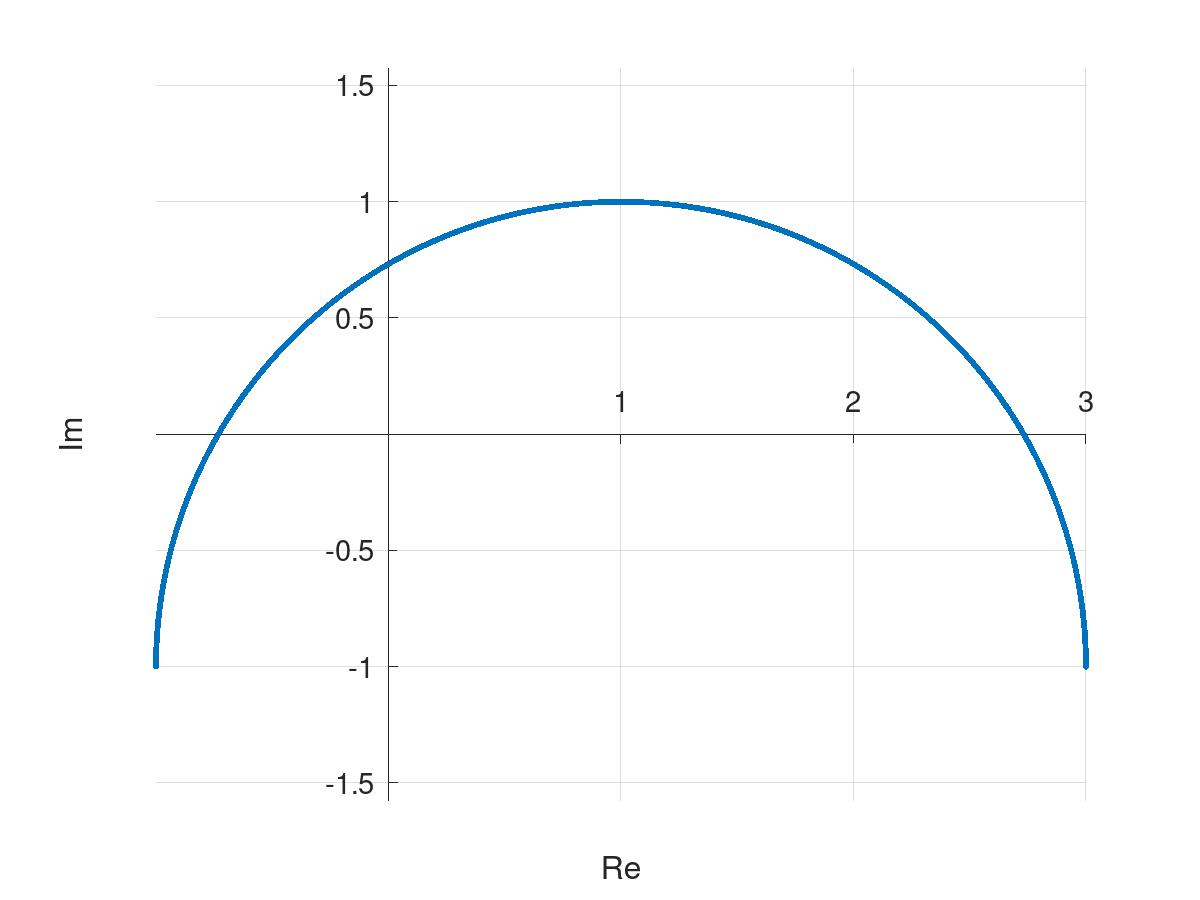
\includegraphics[width=0.55\textwidth]{2b.jpg}
     	\caption{Representaci\'on de $1-i+2e^{i\theta}$, ver Ej. \ref{ej:sol2b}}
		\label{fig:sol2b}
	\end{figure}
\end{enumerate}

% ***********************************************
% 					Ejercicio 3
% ***********************************************
\item 
\begin{enumerate}
	\item   % ****************************************** 3.a
	\textbf{Trayectoria $C_1$} 
	
	La trayectoria C\textsubscript1 la podemos representar de forma param\'etrica 
	partiendo de la funci\'on $y=x$. Le asignamos a $x$ el rol del par\'ametro $t$ 
	haciendo $x=t$, para $0\leq t \leq 1$, y queda $y=t$.
	
	Con lo anterior podemos escribir,
	\begin{equation}
	z = x+iy ~~ \rightarrow ~~ z(t) = t+it=t(1+i).
	\label{eq:3aC1}
	\end{equation}
	Entonces, la funci\'on a la que se le desea calcular la integral es,
	\begin{equation}
		Re\{z\} = x = t. 
	\end{equation}
	Obtenemos la derivada de $z(t)$,
	\begin{equation}
		\dfrac{dz(t)}{dt} = 1+i.
	\end{equation}
	Finalmente, la integral resulta,
	\begin{equation}
		I_1 = \int_0^1 t (1+i) dt = (1+i) \left. \dfrac{t^2}{2} \right|_0^1 = 
		\boxed{\dfrac{1}{2}(1+i)}.
	\end{equation}

	\textbf{Trayectoria $C_2$} \\
	La trayectoria C\textsubscript2  la dividimos en dos tramos.
	
	\textit{Tramo 1}: tomamos $0\leq x \leq 1$ y $y=0$.	Le asignamos a $x$ el rol 
	del par\'ametro $t$ haciendo $x=t$, para $0\leq t \leq 1$.	Con lo anterior 
	podemos escribir,
	\begin{equation}
		z = x+iy ~~ \rightarrow ~~ z(t) = t.
		\label{eq:3a_C2T1}
	\end{equation}
	Entonces, la funci\'on a la que se le desea calcular la integral es,
	\begin{equation}
		Re\{z\} = x = t. 
	\end{equation}
	Obtenemos la derivada de $z(t)$,
	\begin{equation}
		\dfrac{dz(t)}{dt} = 1.
	\end{equation}
	Finalmente, la integral resulta,
	\begin{equation}
		I_{21} = \int_0^1 t dt =  \left.\dfrac{t^2}{2}\right|_0^1 = \dfrac{1}{2}.
	\end{equation}
	
	\textit{Tramo 2}: tomamos $x=1$ y $y=t$ para $0\leq t \leq 1$. Con lo 
	anterior podemos escribir,
	\begin{equation}
		z = x+iy ~~ \rightarrow ~~ z(t) = 1+it.
	\end{equation}
	Entonces, la funci\'on a la que se le desea calcular la integral es,
	\begin{equation}
		Re\{z\} = x = 1. 
	\end{equation}
	Obtenemos la derivada de $z(t)$,
	\begin{equation}
		\dfrac{dz(t)}{dt} = i.
	\end{equation}
	Finalmente, la integral resulta,
	\begin{equation}
		I_{22} = \int_0^1 1\cdot i dt = it |_0^1 = i.
	\end{equation}
	Sumamos los resultados para los dos tramos y obtenemos,
	\begin{equation}
		I_2 = I_{21}+I_{22} = \boxed{\dfrac{1}{2} + i}.
	\end{equation}
	
	\textbf{Trayectoria $C_3$} \\
	La trayectoria C\textsubscript3  la dividimos en dos tramos.
	
	\textit{Tramo 1}: tomamos $x = 0$ y $y=t$, con $0\leq t \leq 1$. Con lo 
	anterior podemos escribir,
	\begin{equation}
	z = x+iy ~~ \rightarrow ~~ z(t) = it.
	\label{eq:3a_C3T1}
	\end{equation}
	Entonces, la funci\'on a la que se le desea calcular la integral es,
	\begin{equation}
	Re\{z\} = x = 0. 
	\end{equation}
	Obtenemos la derivada de $z(t)$,
	\begin{equation}
	\dfrac{dz(t)}{dt} = i.
	\end{equation}
	Finalmente, la integral resulta,
	\begin{equation}
	I_{31} = \int_0^1 0 \cdot i dt = 0.
	\end{equation}

	\textit{Tramo 2}: tomamos $x=t$, para $0\leq t \leq 1$, y $y=1$. Con lo 
	anterior podemos escribir,
	\begin{equation}
	z = x+iy ~~ \rightarrow ~~ z(t) = t+i.
	\label{eq:3a_C3T2}
	\end{equation}
	Entonces, la funci\'on a la que se le desea calcular la integral es,
	\begin{equation}
	Re\{z\} = x = t. 
	\end{equation}
	Obtenemos la derivada de $z(t)$,
	\begin{equation}
	\dfrac{dz(t)}{dt} = 1.
	\end{equation}
	Finalmente, la integral resulta,
	\begin{equation}
	I_{32} = \int_0^1 t\cdot 1 dt = \left. \dfrac{t^2}{2} \right|_0^1 = \dfrac{1}{2}.
	\end{equation}
	
	Sumamos los resultados para los dos tramos y obtenemos,
	\begin{equation}
	I_3 = I_{31}+I_{32} = \boxed{\dfrac{1}{2}}.
	\end{equation}

%% -- 
\begin{profesor}
	\item   % ****************************************** 3.b	
	\textbf{Trayectoria $C_1$} \\
	Se usa la parametrizaci\'on dada en la Ec. \ref{eq:3aC1}. Reemplazando,
	\begin{equation}
	f(z(t)) = t-t-i3t^2 = -i3t^2.
	\end{equation}
	Tomando en cuenta la expresi\'on dada por la Ec. \ref{eq:ht1} se escribe
	\begin{equation}
	I_1 = \int_0^1 -i3t^2(1+i)dt = -i(1+i)(t^3|_0^1 = 1-i.
	\end{equation}
	
	\textbf{Trayectoria $C_3$} \\
	Se resuelve en dos tramos. \\
	\textit{Tramo 1.} Se considera la parametrizaci\'on dada en la Ec. \ref{eq:3a_C3T1}.
	Reemplazando,
	\begin{equation}
	f(z(t)) = t.
	\end{equation}
	Tomando en cuenta la expresi\'on da por la Ec. \ref{eq:ht1} se escribe
	\begin{equation}
	I_{31} = \int_0^1 tidt = i(t^2|_0^1 = \dfrac{i}{2}.
	\end{equation} 
	
	\textit{Tramo 2.} Se considera la parametrizaci\'on dada en la Ec. \ref{eq:3a_C3T2}.
	Reemplazando,
	\begin{equation}
	f(z(t)) = 1-t-i3t^2.
	\end{equation}
	Tomando en cuenta la expresi\'on da por la Ec. \ref{eq:ht1} se escribe
	\begin{equation}
	I_{32} = \int_0^1 (1-t-i3t^2)dt = \left(t-\dfrac{t^2}{2}-it^3\right|_0^1 = 
	\dfrac{1}{2}-i.
	\end{equation}
	Sumando los resultados para los dos tramos resulta,
	\begin{equation}
	I=I_{31}+I_{32}=\boxed{\frac{1}{2}(1-i)}.
	\end{equation}
\end{profesor}
	
\end{enumerate}
% ***********************************************
% 					Ejercicio 4
% ***********************************************
\item  
	Notar que la trayectoria $C_7$ esta definida por la ecuaci\'on de una 
	recta, $y=4x-1$. Por lo que, haciendo $x=t$, puede parametrizarse si se 
	toma $y=4t-1$, o sea que,
	\begin{equation}
	z(t)=x(t)+iy(t)=t+i(4t-1), \quad \forall ~ t_0 \leq t \leq t_1.
	\label{eq:sol4a1}
	\end{equation}	
	Para hallar el rango de variaci\'on del par\'ametro resolvemos las 
	ecuaciones determinadas por los puntos extremos de $C_7$ dados en el 
	enunciado, a saber,
	\begin{equation}
	z(t_0)=t_0+i(4t_0-1)=0-i \rightarrow t_0=0,
	\label{eq:sol4a2}
	\end{equation}	
	\begin{equation}
	z(t_1)=t_1+i(4t_1-1)=1+3i \rightarrow t_1=1.
	\label{eq:sol4a3}
	\end{equation}	
	Por lo que la parametrizaci\'on queda,
	\begin{equation}
	z(t)=t(1+4i)-i, \quad \forall ~ 0 \leq t \leq 1.
	\label{eq:sol4a4}
	\end{equation}
	Derivando la Ec. \ref{eq:sol4a4} obtenemos,
	\begin{equation}
	 \frac{dz(t)}{dt} =1+4i
	\label{eq:sol4a5}
	\end{equation}
	Ahora tenemos todos los elementos para resolver la integral planteada 
	mediante la parametrizaci\'on de la trayectoria. Utilizando la Ec. 
	\ref{eq:ht1} podemos escribir,
	\begin{equation}
	\int_{C_7}^{}(z^2-4zi) dz=\int_{0}^{1}\left[ 
	[t(1+4i)-i]^2-4i[t(1+4i)-i]\right](1+4i)dt,
	\label{eq:sol4a6}
	\end{equation}	
	que es una integral definida de una variable real.
	Operando sobre la Ec.\ref{eq:sol4a6} tenemos,
	\begin{equation}
	\begin{split}
	\int_{C_7}^{}(z^2-4zi) dz&=(1+4i) 
	\int_{0}^{1}\left[t^2(1+4i)^2-2ti(1+4i)-1-4ti(1+4i)-4]\right]dt, \\
	&=(1+4i) \int_{0}^{1}\left[t^2(1+4i)^2-6ti(1+4i)-5]\right]dt,\\
	&=(1+4i) \left|t^3\frac{(1+4i)^2}{3}-t^2\frac{6i(1+4i)}{2}-5t\right|_0^1,\\	
	&=(1+4i) \left[\frac{(1+4i)^2}{3}-3i+7\right],\\
	&=\boxed{\frac{10}{3}+\frac{23}{3}i}.
	\label{eq:sol4a7}
	\end{split}
	\end{equation}		
	
% ***********************************************
% 					Ejercicio 5
% ***********************************************
%% --

\begin{profesor}
\item Le asignamos a $x$ el rol del par\'ametro $t$ haciendo,
	\begin{equation}
		x=t, ~~ 0 \leq t \leq 1.
	\end{equation}
	
	Para la trayectoria definida queda $y=t^2$. Con lo que podemos escribir,
	\begin{equation}
		z = x+iy ~~ \rightarrow ~~ z(t) = t+it^2.
	\end{equation}

	Obtenemos la derivada de $z(t)$,
	\begin{equation}
		\dfrac{dz(t)}{dt} = 1+i2t.
	\end{equation}
	
	La funci\'on a la que se le desea calcular la integral es,
	\begin{equation}
		f[z(t)] = t-it^2+1 = t+1+it^2. 
	\end{equation}
	
	Finalmente, la integral resulta,
	\begin{equation}
		I = \int_0^1 (t+1+it^2)(1+i2t) dt = 1+2i.
	\end{equation}
\end{profesor}

% ***********************************************
% 					Ejercicio 6
% ***********************************************
%% --
\begin{profesor}
\item {Utilizando la Ec. \ref{eq:ht4} podemos dividir la reoluci\'on de la 
integral en tramos como sigue,}

	\begin{equation}
	\oint_{C}z^2dz=\oint_{C_1}z^2dz+\oint_{C_2}z^2dz+\oint_{C_3}z^2dz
	\label{eq:sol6}
 	\end{equation}

	Resolvemos ahora cada tramo por separado.
	
	\textit{Trayectoria $C_1$:}\\
	Esta puede parametrizarse haciendo, $x=-t+1$ e $y=t$ si se considera un 
	intervalo de variaci\'on del par\'ametro $0\leq t \leq 1$. Por lo que 
	podemos escribir,

	\begin{equation}
	z(t)=-t+1+it=t(i-1)+1~ \forall ~ 0 \leq t \leq 1.
	\end{equation}
	
	Obtenemos la derivada de $z(t)$,
	\begin{equation}
	\dfrac{dz(t)}{dt} = i-1.
	\end{equation}
	
	Por lo que la primera integral de la Ec. \ref{eq:sol6} queda,
	\begin{equation}
	\begin{split}
	I_1=\oint_{C_1}z^2dz & = \int_{0}^{1} [t(i-1)+1]^2 (i-1)dt,\\
	& = (i-1) \int_{0}^{1} [t^2(i-1)^2+2t(i-1)+1] dt,\\
	& = (i-1) \left| t^3 \frac{(i-1)^2}{3}+2t^2\frac{(i-1)}{2}+t \right|_0^1,\\
	& = (i-1) \left[\frac{(i-1)^2}{3}+i\right],\\
	\end{split}
	\end{equation}	
	que resulta en,
	\begin{equation}
	I_1=-\frac{1}{3}	-\frac{1}{3}i.
	\label{eq:sol61}
	\end{equation}

	\textit{Trayectoria $C_2$:}\\
	Esta puede parametrizarse haciendo, $x=0$ e $y=-t$ si se considera un 
	intervalo de variaci\'on del par\'ametro $-1\leq t \leq 1$. Por lo que 
	podemos escribir,

	\begin{equation}
	z(t)=-it~ \forall ~ -1 \leq t \leq 1.
	\end{equation}
	
	Obtenemos la derivada de $z(t)$,
	\begin{equation}
	\dfrac{dz(t)}{dt} = -i.
	\end{equation}
	
	Por lo que la segunda integral de la Ec. \ref{eq:sol6} queda,
	\begin{equation}
	\begin{split}
	I_2=\oint_{C_2}z^2dz & = \int_{-1}^{1} (-it)^2(-i)dt,\\
	 & = i\int_{-1}^{1}t^2dt,\\
	\end{split}
	\end{equation}	
	que resulta en,
	\begin{equation}
	I_2=\frac{2}{3}i
	\end{equation}

	\textit{Trayectoria $C_3$:}\\
	Esta puede parametrizarse haciendo, $x=t$ e $y=t-1$ si se considera un 
	intervalo de variaci\'on del par\'ametro $0\leq t \leq 1$. Por lo que 
	podemos escribir,

	\begin{equation}
	z(t)=t+i(t-1)=t(1+i)-i~ \forall ~ 0 \leq t \leq 1.
	\end{equation}
	
	Obtenemos la derivada de $z(t)$,
	\begin{equation}
	\dfrac{dz(t)}{dt} = 1+i.
	\label{eq:sol62}
	\end{equation}
	
	Por lo que la tercera integral de la Ec. \ref{eq:sol6} queda,
	\begin{equation}
	\begin{split}
	I_3=\oint_{C_3}z^2dz & = \int_{0}^{1} [t(1+i)-i]^2 (1+i)dt,\\
	& =  (1+i) \int_{0}^{1}[t^2(1+i)^2-2t(1+i)i-1]dt,\\
	& = (1+i) \left| t^3 \frac{(1+i)^2}{3}-2it^2\frac{(1+i)}{2}-t \right|_0^1,\\
	& = (1+i) \left[\frac{(1+i)^2}{3}-i\right],\\
	\end{split}
	\end{equation}	
	que resulta en,
	\begin{equation}
	I_3=\frac{1}{3}	-\frac{1}{3}i.
	\label{eq:sol63}	
	\end{equation}

Reemplazando Ecs. \ref{eq:sol61}, \ref{eq:sol62} y \ref{eq:sol63} en 
\ref{eq:sol6} encontramos la soluci\'on deseada,

	\begin{equation}
	\oint_{C}z^2dz=I_1+I_2+I_3=-\frac{1}{3}	-\frac{1}{3}i. + \frac{2}{3}i + 
	\frac{1}{3}	-\frac{1}{3}i=0.	
	\end{equation}
\end{profesor}

% ***********************************************
% 					Ejercicio 7
% ***********************************************
\item[7.]
\begin{enumerate}
	% --- a ---
	\item Luego de obtener las ra\'ices del polinomio denominador escribimos: 
	$f(z)=\dfrac{z^2-2z}{z^2+4}=\dfrac{z^2-2z}{(z+i2)(z-i2)}$.
	
	La circunferencia $|z-i|=2$ encierra a la singularidad ubicada en $z_0=i2$. 
	Entonces, seg\'un la Ec. \ref{eq:ht6} tenemos,
	\begin{equation}
	\begin{split}
		\oint_C \dfrac{z^2-2z}{(z+i2)}\dfrac{1}{(z-i2)} dz &= 2\pi i 
		\left| \dfrac{z^2-2z}{(z+i2)} \right|_{z=i2}  \\
		&= 2\pi i \left( \dfrac{(i2)^2-2(i2)}{(i2+i2)} \right)  \\
		&= \boxed{-2\pi (1+i)} 
	\end{split}
	\end{equation}

\begin{profesor}
	% --- b ---
	\item La circunferencia $|z+\frac{1}{2}|=1$ no encierra ninguna de las 
	singularidades, por lo tanto la integral es $I=0$.

	% --- c ---
	\item La circunferencia $|z+1+i|=2$ encierra a la singularidad ubicada en $z_0=-2i$.
	Entonces, seg\'un la Ec. \ref{eq:ht6} tenemos,
	\begin{equation}
	\begin{split}
		\oint_C \dfrac{z^2-2z}{(z-i2)}\dfrac{1}{(z+i2)} dz &= 2\pi i 
		\left| \dfrac{z^2-2z}{(z-i2)} \right|_{z=-i2} \\
		&= 2\pi i \left( \dfrac{(-i2)^2-2(-i2)}{(-i2-i2)} \right) \\
		&= 2\pi i \left( \dfrac{(-4)+4i}{-i4} \right) \\
		&= \boxed{2\pi (1-i)}
	\end{split}
	\end{equation}
\end{profesor}
	
\end{enumerate}

% ***********************************************
% 					Ejercicio 8
% ***********************************************
\item [8.]
\begin{enumerate}
%\item 
\label{ej:sol8a}
	
\item [\textit{b})]
\label{ej:sol8b}
Factorizamos el polinomio en el numerador del integrando mediante una 
diferencia de cuadrados,

	\begin{equation}
	\oint_{C}\frac{e^{3z}}{z^2+\frac{1}{4}}dz=\oint_{C}\frac{e^{3z}}{z^2-(\frac{i}{2})^2}dz=
	\oint_{C}\frac{e^{3z}}{(z-\frac{i}{2})(z+\frac{i}{2})}dz.
	\end{equation}

Notar que el integrando es anal\'itico para todo $z$, excepto en sus polos 
(ceros del denominador). En la Fig. \ref{fig:sol8} puede verse que la 
trayectoria dada,  $C:|z-i|=1$ , encierra \'unicamente al polo en $0+i/2$.

	\begin{figure}[!htbp]
	\centering
	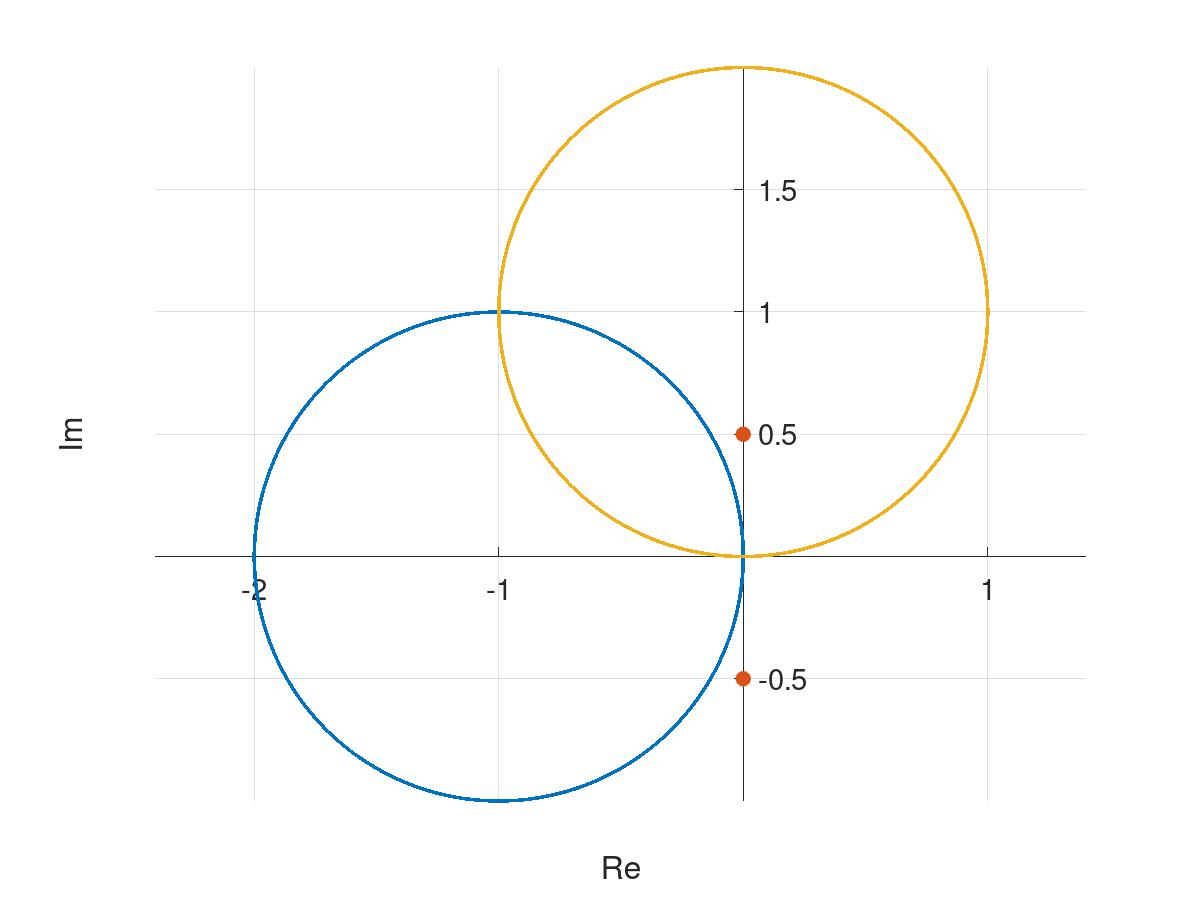
\includegraphics[width=0.6\textwidth]{8a_b.jpg}
	\caption{Trayectorias de integraci\'on de los Ejs. 8a (azul) y 
	8b (amarillo). Se muestran adem\'as los polos del integrando 
	(rojo).}
	\label{fig:sol8}
	\end{figure}

Por lo tanto la aplicaci\'on de la Ec. \ref{eq:ht6} permite resolver la 
integral 
de 
la siguiente manera:

	\begin{equation}
\begin{split}
\oint_{C}\frac{e^{3z}}{(z-\frac{i}{2})(z+\frac{i}{2})}dz&=2\pi i \left| 
\frac{e^{3z}}{z+\frac{i}{2}} \right|_{z=i/2} \\
&=2\pi i \frac{e^{\frac{3}{2}i}}{\frac{i}{2}+\frac{i}{2}} \\
&=2\pi [cos(3/2)+isen(3/2)]\\
&=\boxed{2\pi(0.071+0.997i)}
\end{split}
\end{equation}	

\end{enumerate}

% ***********************************************
% 					Ejercicio 9
% ***********************************************
\item [9.]
\begin{enumerate}
	
	\item Factorizamos el polinomio en el numerador del integrando mediante una 
	diferencia de cuadrados,
	\label{ej:sol9a}
	
	\begin{equation}
	\oint_{C}\frac{1}{z^4-1}dz=\oint_{C}\frac{1}{(z-1)(z-i)(z+1)(z+i)}dz.
	\end{equation}
	
	Notar que el integrando es anal\'itico para todo $z$, excepto en sus polos 
	(ceros del denominador). En la Fig. \ref{fig:sol9} puede verse que la 
	trayectoria dada,  $C:|z+1|=1$ , encierra \'unicamente al polo en $-1$.
	
	\begin{figure}[!htbp]
		\centering
		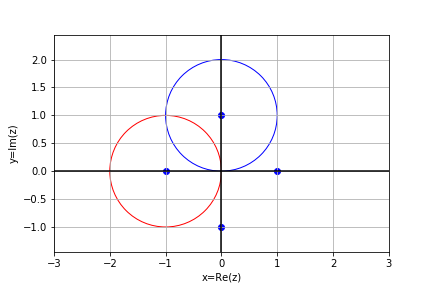
\includegraphics[width=0.6\textwidth]{tp3_9ab.png}
		\caption{Trayectorias de integraci\'on de los Ejs. 9a (rojo) y 
			9b (azul). Se muestran adem\'as los polos del integrando 
			(puntos azules).}
		\label{fig:sol9}
	\end{figure}
	
	Por lo tanto la aplicaci\'on de la Eq. \ref{eq:ht6} permite resolver la 
	integral de	la siguiente manera:
	
	\begin{equation}
	\begin{split}
	\oint_{C}\frac{1}{(z-1)(z-i)(z+1)(z+i)}dz&=2\pi i \left| 
	\frac{1}{(z-1)(z-i)(z+i)} \right|_{z=-1} \\
	&= \frac{2\pi i}{(-1-1)(-1-i)(-1+i)}  \\
	&=\frac{2\pi i}{(-2)[(1^2-i^2)]}  \\
	&=\frac{2\pi i}{(-2)2}\\ 
	&=\boxed{-\frac{\pi i}{2}}
	\end{split}
	\end{equation}	

%	\item
	\label{ej:sol9b}	
\end{enumerate}

% ***********************************************
% 					Ejercicio 10
% ***********************************************
\item [10.]
\label{ej:sol10}
\begin{enumerate}
	\item[\textit{d})] Operamos en el denominador del integrando para hallar su raiz,
	\begin{equation}
	\oint_{C}\frac{z^3}{2z-i}=\oint_{C}\frac{z^3}{2(z-\frac{i}{2})}.
	\end{equation}
    En el la Fig. \ref{fig:sol10} puede verse que la trayectoria dada, $C$, 
    encierra al polo ubicado en $0+i/2$. La aplicaci\'on de la Ec. 
    \ref{eq:ht6} permite entonces resolver la integral de la siguiente manera,
	\begin{equation}
	\oint_{C}\frac{z^3}{2(z-\frac{i}{2})}=2\pi i 
	\left|\frac{z^3}{2}\right|_{z=i/2}=\boxed{\frac{\pi}{8}}
	\end{equation}
	\begin{figure}[!htbp]
		\centering
		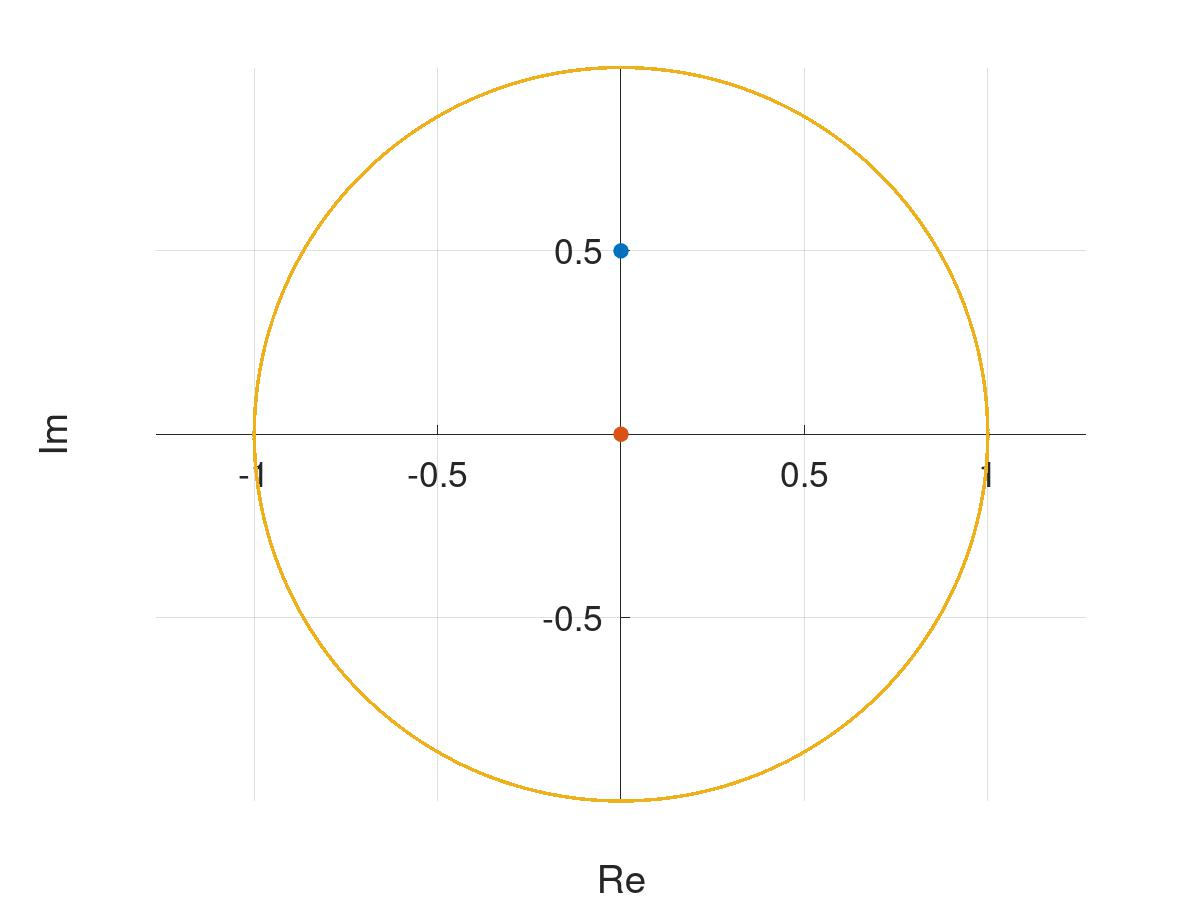
\includegraphics[width=0.5\textwidth]{10.jpg}
		\caption{Trayectoria de integraci\'on del Ej. 10 (amarillo) 
		junto al polo del integrando (punto azul)  y su cero (punto rojo).}
		\label{fig:sol10}
	\end{figure}	
\end{enumerate}

% ***********************************************
% 					Ejercicio 11
% ***********************************************
\item [11.]
Para el c\'alculo de las integrales, escribimos la Ec. \ref{eq:derivadafanalitica} 
de la siguiente forma,
\begin{equation}\label{eq:integralderivada}
I=\oint_C\dfrac{f(z)}{(z-z_0)^{n+1}}dz=\dfrac{2\pi i}{n!}f^{(n)}(z_0).
\end{equation}

\begin{enumerate}
% --- (a) ---
\item $f(z)=\dfrac{z^2}{(z-i)^2}$ \\
\label{ej:sol11a}
\textbf{Trayectoria $C: |z+1|=2$}\\ 
La circunferencia $|z+1|=2$ encierra a la singularidad en $z_0=i$, ver Fig. \ref{fig:sol11a}. Entonces,
\begin{align}
\oint_C \dfrac{z^2}{(z-i)^{2}}dz&=\dfrac{2\pi i}{1!}\left| \dfrac{d}{dz}(z^2)\right|_{z=i}&\\
								&= 2\pi i (2z|_{z=i} = \boxed{-4\pi}
\end{align}
\begin{figure}[!htbp]
	\centering
	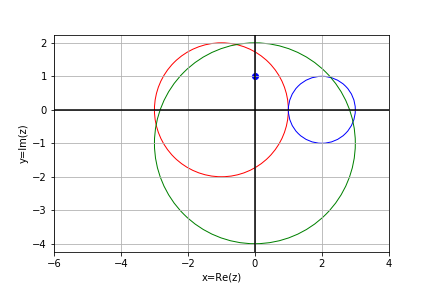
\includegraphics[width=0.6\textwidth]{tp3_11a.png}
	\caption{Trayectorias de integraci\'on del Ej. 11a (c�rculos de diferentes colores) 
		junto al polo doble del integrando (punto en azul).}
	\label{fig:sol11a}
\end{figure}

\textbf{Trayectoria $C: |z-2|=1$}\\ 
La circunferencia $|z-2|=1$ no encierra ninguna singularidad, ver Fig. \ref{fig:sol11a}. Entonces $ \boxed{I=0}$.

\textbf{Trayectoria $C: |z+i|=3$}\\ 
La circunferencia $|z+i|=3$ encierra a la singularidad en $z_0=i$, ver Fig. \ref{fig:sol11a}. Entonces,
\begin{align}
\oint_C \dfrac{z^2}{(z-i)^{2}}dz&=\dfrac{2\pi i}{1!}\left| \dfrac{d}{dz}(z^2)\right|_{z=i}&\\
								&= 2\pi i (2z|_{z=i} = \boxed{-4\pi}
\end{align}

%% --- (b) ---
\begin{profesor}
\item $f(z)=\dfrac{z^4}{(z-3i)^3}$ \\
$C: |z|=4$\\ 
La circunferencia $|z|=4$ encierra a la singularidad en $z_0=3i$. Entonces,
\begin{align}
\oint_C \dfrac{z^4}{(z-3i)^{3}}dz&=\dfrac{2\pi i}{2!}\left[ \dfrac{d^2}{dz^2}(z^4)\right]_{z=3i}&\\
								&= \pi i (12z^2|_{z=3i} = \boxed{-108\pi i}
\end{align}

$C: |z+2|=3$\\ 
La circunferencia $|z+2|=3$ no encierra ninguna singularidad. Entonces $I=0$.

$C: |z-i|=4$\\ 
La circunferencia $|z-i|=4$ encierra a la singularidad en $z_0=3i$. Entonces,
\begin{align}
\oint_C \dfrac{z^4}{(z-3i)^{3}}dz&=\dfrac{2\pi i}{2!}\left[ \dfrac{d^2}{dz^2}(z^4)\right]_{z=3i}&\\
								&= \pi i (12z^2|_{z=3i} = \boxed{-108\pi i}
\end{align}
***

% --- (c) ---
\item $f(z)=\dfrac{4z^3-3z}{(z+2)^3}$ \\
$C: |z|=4$\\ 
La circunferencia $|z|=4$ encierra a la singularidad en $z_0=-2$. Entonces,
\begin{align}
\oint_C \dfrac{4z^3-3z}{(z+2)^3}dz&=\dfrac{2\pi i}{2!}\left[ \dfrac{d^2}{dz^2}(4z^3-3z)\right]_{z=-2}&\\
								&= \pi i (24z|_{z=-2} = \boxed{-48\pi i}
\end{align}

$C: |z-i|=3$\\ 
La circunferencia $|z-i|=3$ encierra a la singularidad en $z_0=-2$. Entonces,
\begin{align}
\oint_C \dfrac{4z^3-3z}{(z+2)^3}dz&=\dfrac{2\pi i}{2!}\left[ \dfrac{d^2}{dz^2}(4z^3-3z)\right]_{z=-2}&\\
								&= \pi i (24z|_{z=-2} = \boxed{-48\pi i}
\end{align}

$C: |z-2|=3$\\ 
La circunferencia $|z-2|=3$ no encierra ninguna singularidad. Entonces $I=0$.\\
***

\item

% --- (e) ---
\item $f(z)=\dfrac{Sinh(z)}{z^3}$ \\
$C: |z-1|=4$\\ 
La $C$ encierra a la singularidad en $z_0=0$. Entonces,
\begin{align}
	\oint_C\dfrac{Sinh(z)}{z^3}dz&=\dfrac{2\pi i}{2!}\left[ \dfrac{d^2}{dz^2}Sinh(z)\right]_{z=0}&\\
	&= \pi i (Sinh(z)|_{z=0} = \boxed{0}
\end{align}

$C: |z-2|=3$\\ 
La $C$ encierra a la singularidad en $z_0=0$. Por lo que el resultado es el mismo:
\begin{align}
\oint_C\dfrac{Sinh(z)}{z^3}dz& = \boxed{0}
\end{align}

$C: |z-2i|=3$\\ 
La $C$ encierra a la singularidad en $z_0=0$. Por lo que el resultado es el mismo:
\begin{align}
\oint_C\dfrac{Sinh(z)}{z^3}dz& = \boxed{0}
\end{align}
***
\end{profesor}

\end{enumerate}


%------------------------
\end{enumerate}
\begin{center}
	---------------------------------------
\end{center}
\end{document}
